% fixture: tikz/curves
% tier: T3
% engine: document
% specials: compare
% covers: .. controls .. curves (one or two supports, relative ones, to a node's border, .. cycle, labels on them, sloped), to[out=,in=] and bend left/right (relative curves between nodes, looseness, min distance, every curve to), edges (after a point and a node, with options, labels and bends), pins (pin distance, pin edge, every pin edge), arcs (both syntaxes, ellipses, delta angle, labels on an arc), grids (step, xstep, ystep), coordinate options ([shift=…], [xshift=…])
% issue: #326
\documentclass{article}
\usepackage{tikz}
\begin{document}
\noindent Curves: 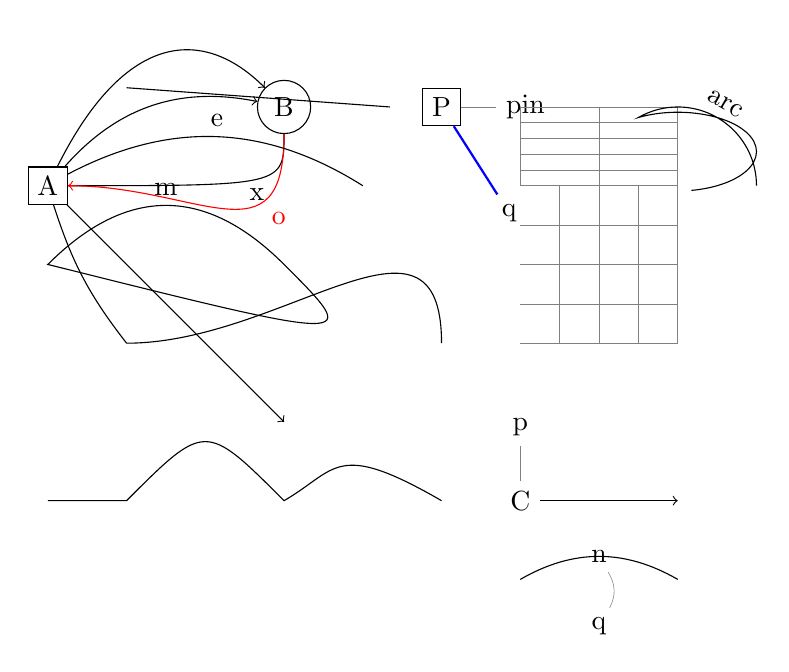
\begin{tikzpicture}
  \node[draw] (a) {A};
  \node[draw,circle] (b) at (3,1) {B};
  \draw[->] (a) .. controls (1,2) and (2,2) .. (b);
  \draw (b) .. controls +(0,-1) .. (a) node[midway,below] {x};
  \draw (0,-1) .. controls (1,0) and (2,0) .. node[sloped,above] {m} (3,-1) .. controls (4,-2) .. cycle;
  \draw[->] (a) to[bend left] (b);
  \draw[->,red] (b) to[out=-90,in=0,looseness=1.5] node[pos=0.3,auto] {o} (a);
  \draw (a) to[bend right=10] +(1,-2) to[out=0,in=90,min distance=2cm] (5,-2);
  \draw (a) edge[->] (3,-3) edge[bend left] node[above] {e} (4,0);
  \node[draw,pin=right:pin,pin={[pin edge={blue,thick},pin distance=1cm]-60:q}] at (5,1) {P};
  \draw[help lines,step=5mm] (6,-2) grid (8,0) (6,0) grid[xstep=1cm,ystep=2mm] (8,1);
  \draw (9,0) arc (0:120:1) node[midway,sloped,above] {arc} arc[start angle=120,delta angle=-200,x radius=1,y radius=0.5];
  \draw ([shift={(1,1)}]a.north) -- ([xshift=1cm]b.east);
  \draw (0,-4) -- +(1,0) .. controls +(1,1) .. (3,-4) to[bend left,in looseness=2] (5,-4);
  \node[pin=above:p] (c) at (6,-4) {C} edge[->] (8,-4);
  \draw (6,-5) to[bend left] node[pin=below:q] {n} (8,-5);
\end{tikzpicture}
\end{document}
